\section{Analiza zachowania wyuczonych polityk}
\label{sec:wyniki-zachowanie-polityk}

W trakcie analizy decyzji podejmowanych przez wybrane konfiguracje DQN i REINFORCE 
zaobserwowałem u części modeli REINFORCE
zjawisko nazywane kolapsem polityki (ang. \emph{policy collapse}) albo przedwczesną
zbieżnością do rozwiązania deterministycznego. Polega ono na tym, że
polityka przestaje zależeć od obserwowanego stanu i niezależnie od
niego wybiera zawsze tę samą akcję. 

Według Volodymyra Mniha i współautorów, dodanie regularyzacji entropii
polityki do funkcji celu poprawia eksplorację poprzez ograniczanie
przedwczesnej zbieżności do suboptymalnych, deterministycznych
polityk \cite{mnih_a3c_2016}.
Jak opisałem w podrozdziale~\ref{sec:policy-gradient-reinforce},
zastosowana w tej pracy konfiguracja REINFORCE nie wykorzystuje ani
regularyzacji entropii, ani baseline'u. W szczególności brak
regularyzacji entropii oznacza, że metoda nie ma mechanizmu
ograniczającego przedwczesną zbieżność do polityki deterministycznej.

Aby ocenić skalę tego zjawiska, dla każdej z ośmiu podstawowych
konfiguracji sprawdziłem, dla ilu z pięciu seedów wybierana akcja
przed flopem była identyczna we wszystkich 100\,000 rozdaniach
końcowej ewaluacji, niezależnie od obserwowanego stanu. W praktyce
mierzę więc degenerację decyzji przed flopem. Jeżeli zdegenerowaną
akcją jest \texttt{BET\_4X}, rozdanie kończy się natychmiast
rozstrzygnięciem, więc pozostała część polityki, dotycząca flopu
i rivera, nie jest w takim rozdaniu w ogóle wykorzystywana, a
zaobserwowany kolaps decyzji preflop jest równoważny kolapsowi całej
ścieżki decyzyjnej. Dla żadnej
z czterech konfiguracji DQN nie zaobserwowałem takiej degeneracji.
Dla REINFORCE zjawisko to okazało się natomiast dominujące, co
przedstawiam w tabeli~\ref{tab:reinforce-collapse-counts}.

\begin{table}[htbp]
    \centering
    \caption{Liczba seedów REINFORCE z polityką zdegenerowaną do
    jednej akcji przed flopem, spośród pięciu, po 50\,000 epizodów}
    \label{tab:reinforce-collapse-counts}
    \begin{tabular}{llr}
        \toprule
        Reprezentacja & Nagroda & Zdegenerowane seedy \\
        \midrule
        RAW & zysk netto & 3 / 5 \\
        RAW & skalowana & 5 / 5 \\
        FEATURES & zysk netto & 5 / 5 \\
        FEATURES & skalowana & 2 / 5 \\
        \bottomrule
    \end{tabular}
\end{table}

W piętnastu spośród dwudziestu przebiegów REINFORCE zaobserwowałem
degenerację decyzji przed flopem do jednej akcji. Nie jest to więc
wyjątek dotyczący jednej konfiguracji, lecz częsty wynik w całym
zbiorze przebiegów REINFORCE. Co istotne, konfiguracja REINFORCE FEATURES ze
skalowaną funkcją nagrody, która osiągnęła najwyższe średnie EV
spośród wariantów REINFORCE, jest jednocześnie tą, w której
degeneracja wystąpiła najrzadziej. Dalszą analizę zachowania
prowadzę właśnie na tej konfiguracji, ponieważ zawiera ona
jednocześnie modele zdegenerowane i zróżnicowane, co pozwala
porównać obie grupy w ramach tego samego zestawu seedów
treningowych.

Na rysunku~\ref{fig:reinforce-action-profiles} przedstawiam rozkład
akcji pięciu modeli tej konfiguracji po rozszerzeniu treningu do
100\,000 epizodów. Na osi poziomej znajduje się udział poszczególnych
akcji w końcowej ewaluacji, a na osi pionowej pięć seedów, każdy pasek
przedstawia pełny rozkład akcji jednego modelu. Trzy z pięciu pasków
składają się z wielu kolorów odpowiadających różnym akcjom, natomiast
dwa są jednokolorowe na całej długości.

\begin{figure}[htbp]
    \centering
    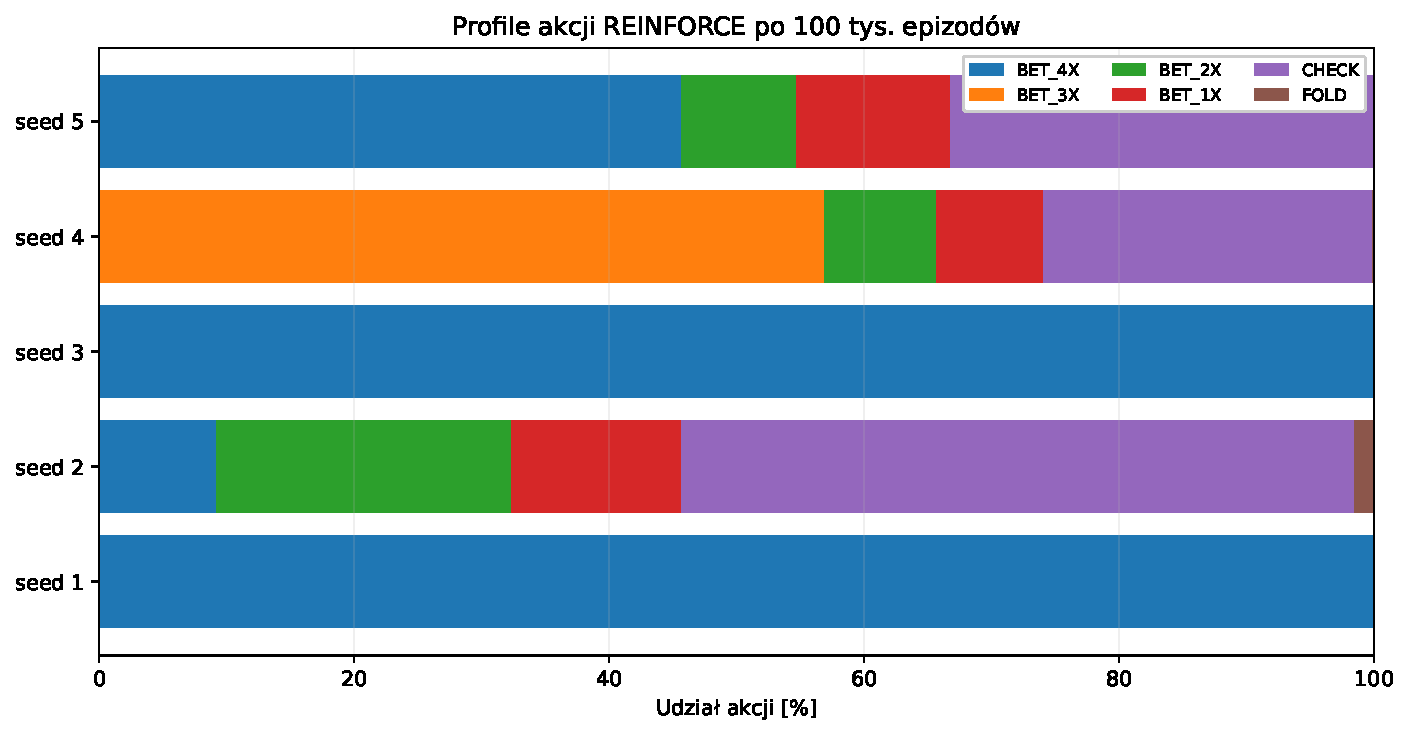
\includegraphics[
        width=\textwidth
    ]{../experiments/results/final_analysis/09_reinforce_action_profiles.pdf}
    \caption{Profile akcji pięciu modeli REINFORCE FEATURES ze
    skalowaną funkcją nagrody}
    \label{fig:reinforce-action-profiles}
\end{figure}

Profile poszczególnych seedów różnią się wyraźnie. Dwa z pięciu
modeli wybierały akcję \texttt{BET\_4X} we wszystkich 100\,000
rozdaniach końcowej ewaluacji. Oznacza to, że polityka tych modeli
uległa degeneracji do bardzo prostej strategii, w której decyzja
przed flopem przestała zależeć od obserwowanego stanu gry.

Pozostałe przebiegi prowadziły do bardziej zróżnicowanych polityk,
które podejmowały również decyzje zależne od kolejnych faz rozdania.
Wyjaśnia to część wysokiej zmienności wyników REINFORCE pomiędzy
seedami. Ta sama konfiguracja treningowa może prowadzić zarówno do
polityki wykorzystującej informacje ze stanu, jak i do rozwiązania
zdominowanego przez jedną akcję.

Zwiększenie budżetu treningowego do 100\,000 epizodów nie
usunęło jednak tego zjawiska. Dwa seedy pozostające w prostej polityce po
50\,000 epizodów nie zmieniły jej również podczas dalszego treningu.
Oznacza to, że sam wzrost liczby epizodów nie wystarczył do
wyprowadzenia tych przebiegów z osiągniętego rozwiązania.

Analizowałem też zachowania agentów poprzez porównanie rozkładu akcji na
kolejnych fazach rozdania. Na rysunku~\ref{fig:action-funnel}
przedstawiam ten rozkład dla agentów Random i RuleBased oraz
najlepszych walidacyjnie konfiguracji DQN i REINFORCE. Trzy panele
odpowiadają preflopowi, flopowi i riverowi, oś pozioma w każdym z nich
przedstawia udział poszczególnych akcji wśród rozdań, które faktycznie
dotarły do danej fazy, a przy panelach flopu i riveru dodatkowo
podałem, jaki odsetek wszystkich rozdań do nich dotarł. Dla DQN
i REINFORCE rozdania pochodzą ze wszystkich pięciu seedów danej
konfiguracji, a nie z jednego wybranego przebiegu. REINFORCE
dociera do riveru w zaledwie 9\% rozdań, podczas gdy dla DQN odsetek
ten wynosi 54\%. Jedną z głównych przyczyn tej różnicy jest częste
wykonywanie zakładu już przed flopem, po którym dalsze decyzje gracza
nie są wymagane.

\begin{figure}[htbp]
    \centering
    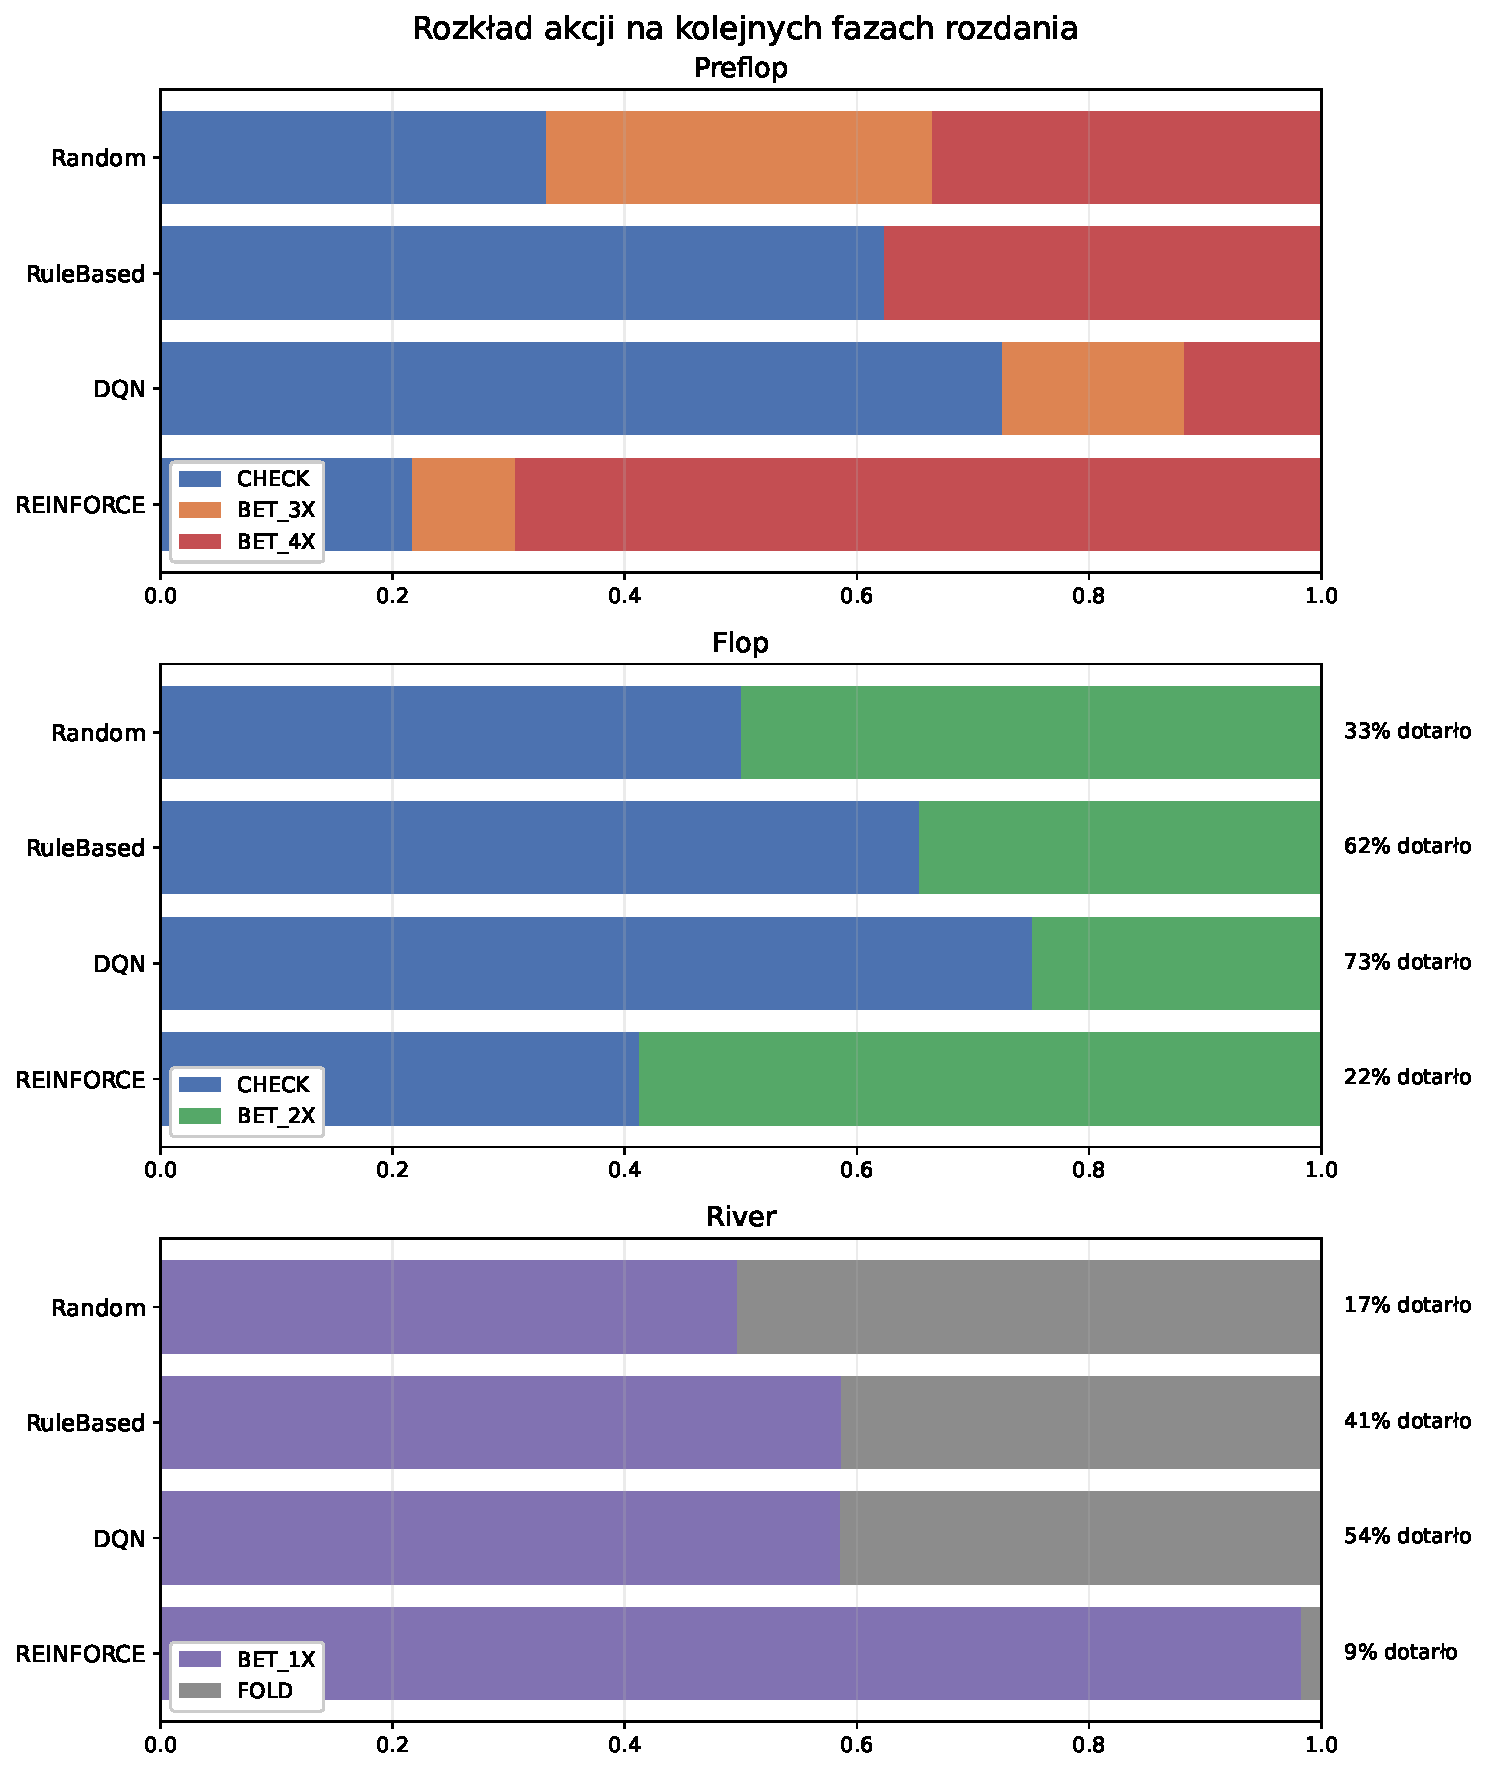
\includegraphics[
        width=\textwidth
    ]{../experiments/results/final_analysis/20_action_funnel_by_street.pdf}
    \caption{Rozkład akcji na kolejnych fazach rozdania}
    \label{fig:action-funnel}
\end{figure}

Przeanalizowałem również zachowanie agentów poprzez porównanie decyzji przed
flopem dla poszczególnych układów początkowych. Na
rysunku~\ref{fig:preflop-range-chart} przedstawiam dominujące decyzje
agenta regułowego oraz wybranych walidacyjnie konfiguracji DQN
i REINFORCE. Trzy panele odpowiadają trzem strategiom, a układ
trzynastu na trzynaście pól w każdym z nich odpowiada wszystkim
kombinacjom dwóch kart początkowych, uporządkowanym według rangi,
kolor pola oznacza dominującą akcję wybraną dla danego układu. Dla DQN
i REINFORCE decyzje pochodzą ze wszystkich pięciu seedów danej
konfiguracji, a nie z jednego wybranego przebiegu.
Agent regułowy tworzy wyraźny, przekątny podział pól, natomiast
u konfiguracji RL taki podział jest znacznie słabiej widoczny albo
nie występuje wcale.

\begin{figure}[htbp]
    \centering
    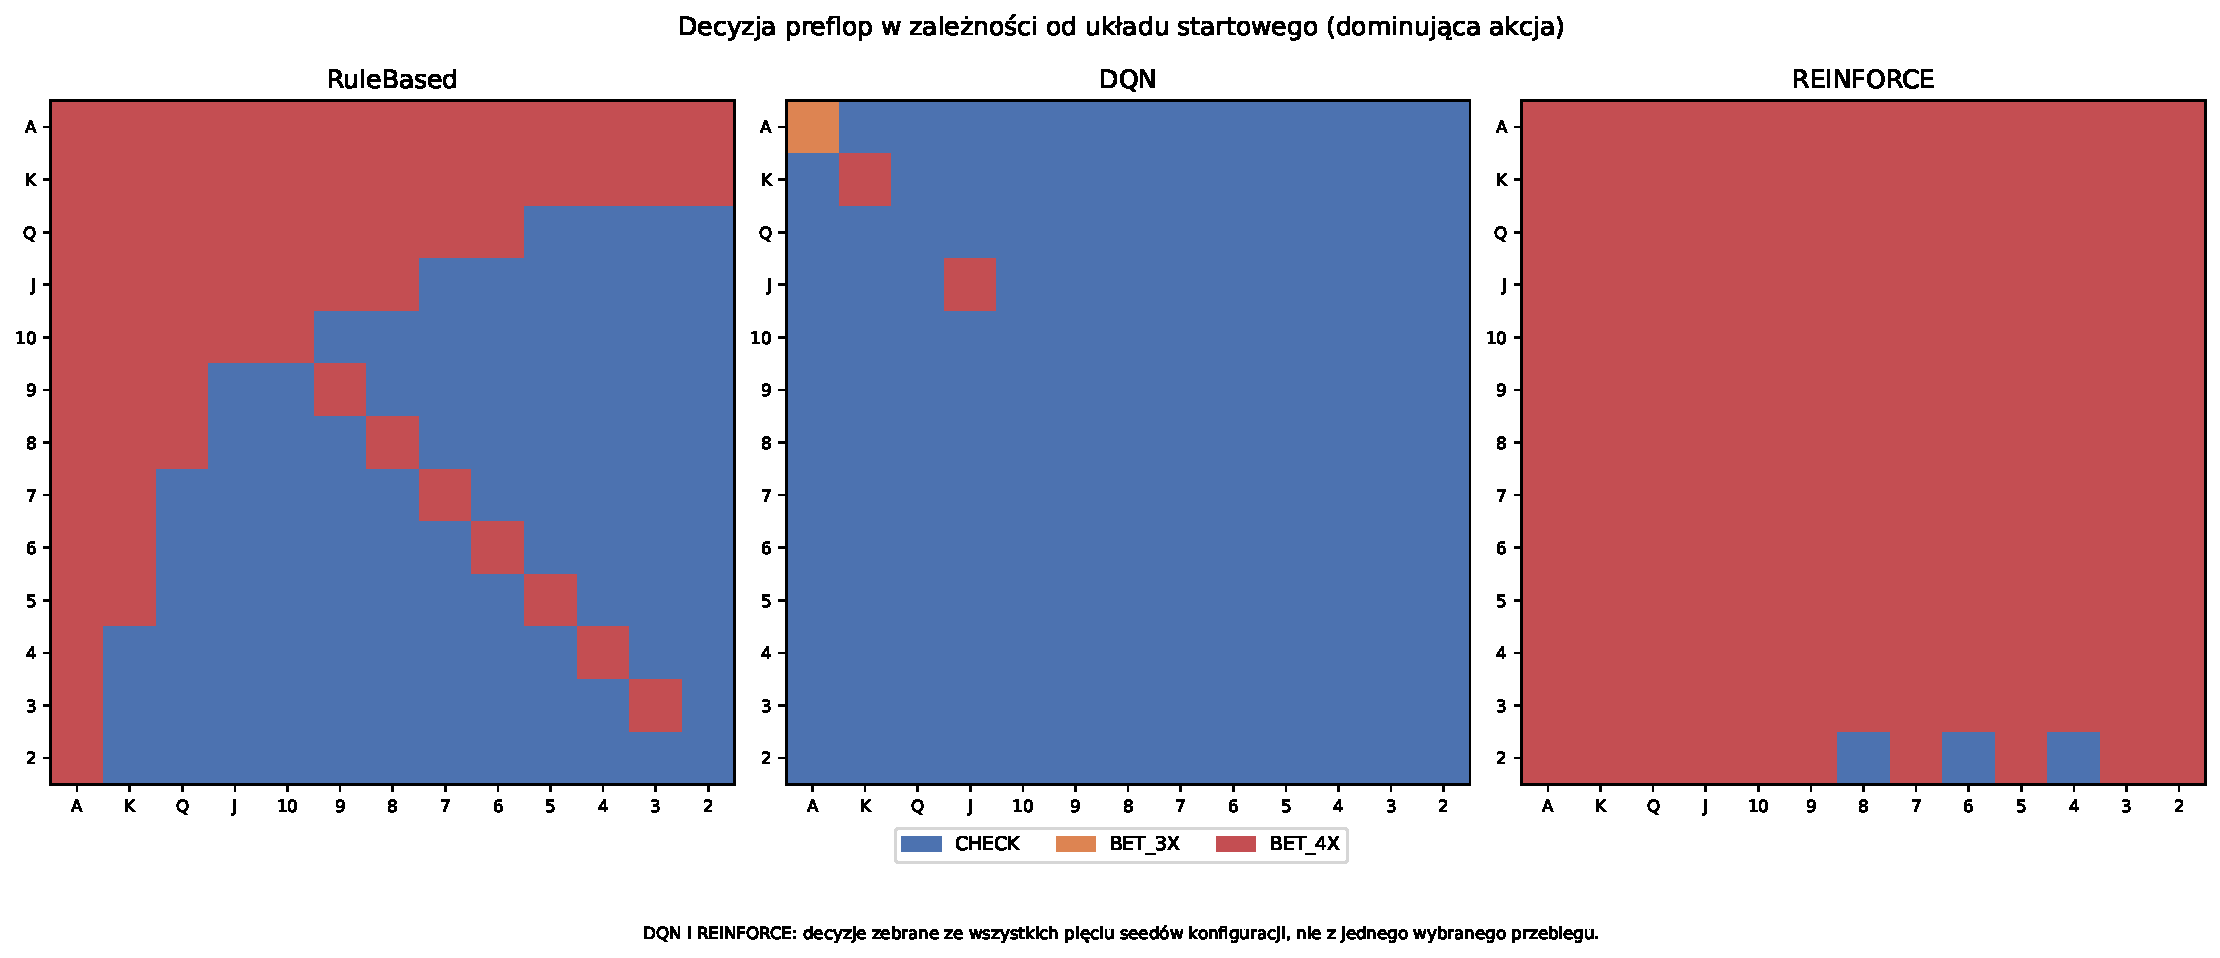
\includegraphics[
        width=0.6\textwidth
    ]{../experiments/results/final_analysis/18_preflop_range_chart.pdf}
    \caption{Dominujące decyzje przed flopem w zależności od układu
    dwóch kart początkowych}
    \label{fig:preflop-range-chart}
\end{figure}

Muszę zaznaczyć, że agent regułowy posiada wyraźnie zdefiniowany obszar układów
początkowych, dla których wykonuje zakład \texttt{BET\_4X}, zgodny
z regułami strategii opisanymi w
rozdziale~\ref{sec:agent-regulowy}. Nauczone polityki tworzą inne
granice decyzyjne, wynikające wyłącznie z procesu optymalizacji
oczekiwanej nagrody.

Porównanie pokazuje, że modele RL nie odtworzyły wprost strategii
agenta regułowego. Jednocześnie ich zachowanie nie jest równoważne
strategii losowej. Szczególnie dla lepszych konfiguracji widoczne są
powtarzalne zależności pomiędzy układem początkowym i wybieraną akcją.
Oznacza to, że w trakcie treningu modele nauczyły się wykorzystywać
część informacji zawartej w obserwowanym stanie, mimo że końcowa
jakość strategii pozostawała niższa od jakości agenta regułowego.
